\textbf{3D Scene Perception:}
3D scene perception is widely studied in computer vision, which can be divided into three mainstream tasks: semantic segmentation~\cite{qi2017pointnet,qi2017pointnet++,graham20183d,choy20194d}, object detection~\cite{hou20193d,Qi_2019_ICCV,rukhovich2022fcaf3d,wang2022cagroup3d} and instance segmentation~\cite{yi2019gspn,jiang2020pointgroup,vu2022softgroup,schult2022mask3d,kolodiazhnyi2023top}.
As we focus on the feature extraction of 3D scene in this work, we mainly discuss the backbone of 3D scene perception networks. Due to the unordered property of point cloud data, voxelizing the points and applying convolution on 3D grids is a natural solution~\cite{chang2015shapenet,qi2016volumetric}.
However, the computational cost and memory requirement both increase cubically with voxel resolution, which is inefficient.
PointNet~\cite{qi2017pointnet} is the pioneer work which directly extracts feature representations from raw point clouds. PointNet++ proposes set abstraction and feature propagation operation based on PointNet, which helps learning more detailed local geometric information. As the furthest point sampling operation in PointNet++ is time consuming, PV-CNN~\cite{liu2019point} converts point clouds to low-resolution voxels and apply 3D convolution to efficiently aggregate local features. Another way to extract high-quality 3D features is sparse convolution~\cite{graham2014spatially,engelcke2017vote3deep}, which voxelizes the point clouds but only apply 3D convolution on non-empty voxels. To further improve the efficiency of sparse CNNs, submanifold sparse convolution~\cite{graham20183d,choy20194d} is introduced, which only conducts convolution when the center of kernel slides over active sites and keeps the same level of sparsity throughout the network. However, these methods are designed for offline 3D scene perception, which is not able to process a streaming RGB-D video at real time.
% Our module can be inserted into mainstream backbones of various tasks to empower them with temporal modeling ability.

\begin{figure*}[t]
    \centering
    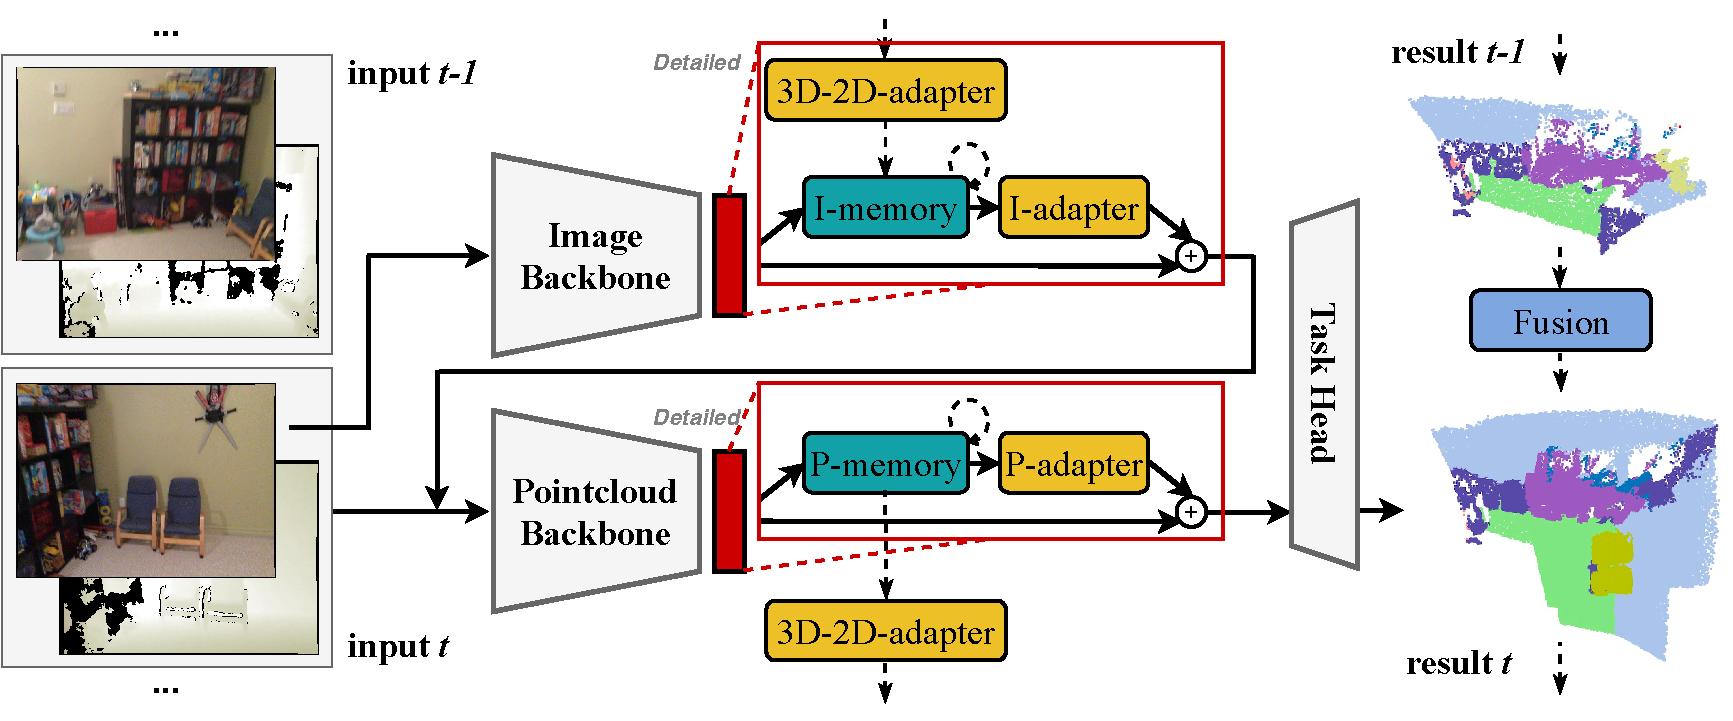
\includegraphics[width=0.9\linewidth]{figures/over-arch-double2.pdf}
    \caption{Overall architecture of our approach. We insert memory-based adapters after image and point cloud backbones, which cache the extracted features in memory over time and perform temporal aggregation. 3D-to-2D adapter is proposed to further exploit inter-modal temporal information. 
    % The orange boxes highlight the effect of temporal modeling, where the predictions are gradually improved as more and more frames are fused in. 
    Solid lines indicate operations within a single frame, while dashed lines indicate temporal operations.}
    \label{over-arch}
\end{figure*}

\textbf{Streaming Data Analysis:}
As the input for online 3D scene perception model is streaming RGB-D video, we review the streaming data analysis methods for both image and point cloud domains.
In 2D vision, many works~\cite{carreira2018massively,dai2019transformer,kondratyuk2021movinets} extend causal convolution~\cite{oord2016wavenet} to streaming videos, where a stream buffer is devised to cache previous frames and 3D causal convolution is applied to unidirectionally aggregate spatial-temporal information. 
TSM~\cite{lin2019tsm} utilizes a more efficient shift mechanism, where a proportion of channels of previous image features are shifted to the next frame. Then the spatial-temporal information can be efficiently aggregated by 2D convolution. Our image adapter also utilizes channel shift for efficient temporal modeling. Differently, TSM is trained from scratch where the network can learn how to model temporal information according to the shift proportion. While we reorganize the channels and adopt channel shift in a plug-and-play adapter to empower image backbone with temporal modeling ability.
However, as 2D streaming videos contain less helpful information for real world applications like robotic navigation~\cite{chaplot2020object,zhang20233d} and manipulation~\cite{Mousavian_2019_ICCV}, increasing attention has been paid to 3D streaming RGB-D video analysis.
A natural solution is to first process 2D images and then project the predictions to 3D point clouds, which is followed by a fusion step to merge the predictions from different frames~\cite{mccormac2017semanticfusion,narita2019panopticfusion}.
Fusion-aware 3D-Conv~\cite{zhang2020fusion} and SVCNN~\cite{huang2021supervoxel} maintain the information of previous frames in 3D space and conduct point-based convolution to fuse the 3D features for semantic segmentation. INS-CONV~\cite{liu2022ins} extends sparse convolution to incremental CNN to efficiently extract global 3D features for semantic and instance segmentation.
Differently, our approach empowers offline model with online perception ability by image and point cloud memory-based adapters, which fully exploits the multimodal temporal relations.